% Architecture diagram for Nephtys — standalone compilable TikZ figure.
% Compile with: pdflatex fig_architecture.tex
\documentclass[border=6pt]{standalone}
\usepackage[T1]{fontenc}
\usepackage{lmodern}
\usepackage{tikz}
\usetikzlibrary{positioning, arrows.meta, fit, calc, decorations.pathreplacing, backgrounds}

\definecolor{sensorblue}{HTML}{4A90D9}
\definecolor{conngreen}{HTML}{27AE60}
\definecolor{pipeorng}{HTML}{E67E22}
\definecolor{natspurp}{HTML}{8E44AD}
\definecolor{cloudgray}{HTML}{6C7A89}
\definecolor{edgebg}{HTML}{FDF6EC}

\begin{document}
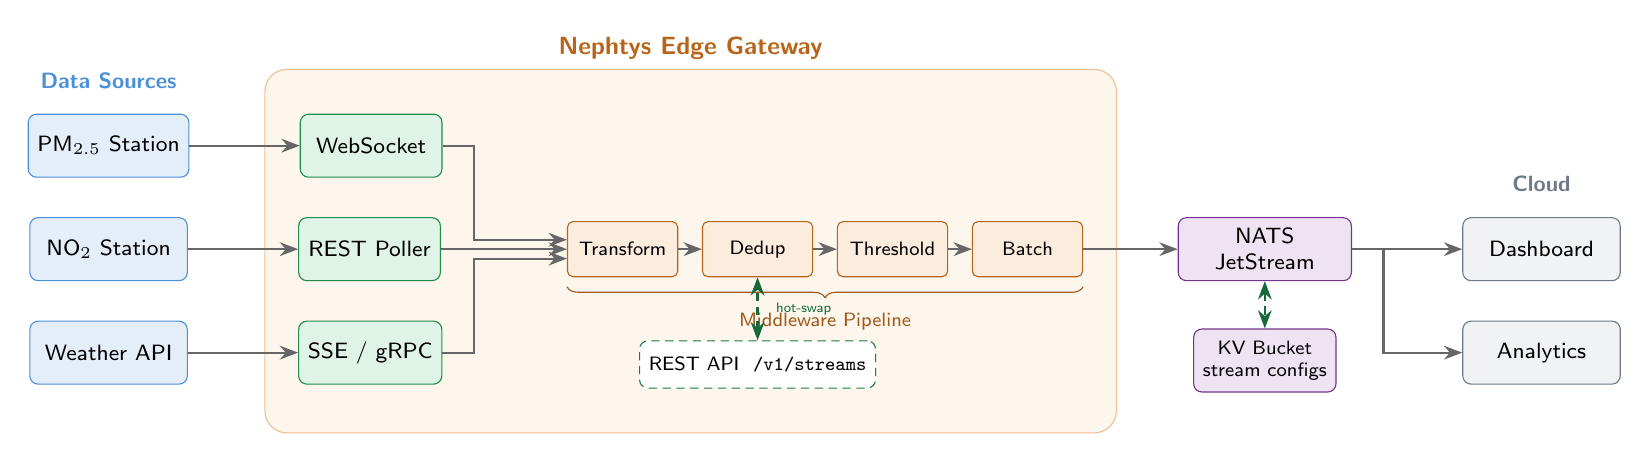
\begin{tikzpicture}[
    >=Stealth,
    every node/.style={font=\sffamily\small},
    sensor/.style={
      rectangle, rounded corners=3pt, draw=sensorblue, fill=sensorblue!15,
      minimum width=2.0cm, minimum height=0.8cm, align=center,
      font=\sffamily\footnotesize
    },
    conn/.style={
      rectangle, rounded corners=3pt, draw=conngreen!80!black, fill=conngreen!15,
      minimum width=1.8cm, minimum height=0.8cm, align=center,
      font=\sffamily\footnotesize
    },
    mw/.style={
      rectangle, rounded corners=2pt, draw=pipeorng!80!black, fill=pipeorng!15,
      minimum width=1.4cm, minimum height=0.7cm, align=center,
      font=\sffamily\scriptsize
    },
    broker/.style={
      rectangle, rounded corners=3pt, draw=natspurp!80!black, fill=natspurp!15,
      minimum width=2.2cm, minimum height=0.8cm, align=center,
      font=\sffamily\footnotesize
    },
    cloud/.style={
      rectangle, rounded corners=3pt, draw=cloudgray, fill=cloudgray!10,
      minimum width=2.0cm, minimum height=0.8cm, align=center,
      font=\sffamily\footnotesize
    },
    api/.style={
      rectangle, rounded corners=3pt, draw=conngreen!70!black,
      fill=white, minimum width=1.8cm, minimum height=0.6cm,
      align=center, font=\sffamily\scriptsize, densely dashed
    },
    arr/.style={->, thick, color=black!60},
    harr/.style={<->, thick, color=conngreen!60!black, densely dashed},
  ]

  % ============ COLUMN 1: Data Sources ============
  \node[sensor]                  (s1) {PM$_{2.5}$ Station};
  \node[sensor, below=0.5cm of s1] (s2) {NO$_2$ Station};
  \node[sensor, below=0.5cm of s2] (s3) {Weather API};
  \node[above=0.2cm of s1, font=\sffamily\footnotesize\bfseries, text=sensorblue]
    {Data Sources};

  % ============ COLUMN 2: Connectors ============
  \node[conn, right=1.4cm of s1] (c1) {WebSocket};
  \node[conn, right=1.4cm of s2] (c2) {REST Poller};
  \node[conn, right=1.4cm of s3] (c3) {SSE / gRPC};

  % ============ COLUMN 3: Pipeline (on the c2 row) ============
  \node[mw, right=1.6cm of c2] (m1) {Transform};
  \node[mw, right=0.3cm of m1]  (m2) {Dedup};
  \node[mw, right=0.3cm of m2]  (m3) {Threshold};
  \node[mw, right=0.3cm of m3]  (m4) {Batch};

  % ============ REST API (below pipeline) ============
  \node[api, below=0.8cm of m2] (api) {REST API~~\texttt{/v1/streams}};

  % ============ COLUMN 4: NATS ============
  \node[broker, right=1.2cm of m4] (nats) {NATS\\JetStream};
  \node[broker, below=0.6cm of nats, minimum width=1.8cm,
        font=\sffamily\scriptsize] (kv) {KV Bucket\\{\scriptsize stream configs}};

  % ============ COLUMN 5: Cloud ============
  \node[cloud, right=1.4cm of nats]  (cl1) {Dashboard};
  \node[cloud, below=0.5cm of cl1]   (cl2) {Analytics};
  \node[above=0.2cm of cl1, font=\sffamily\footnotesize\bfseries, text=cloudgray]
    {Cloud};

  % ============ Edge Gateway background ============
  \begin{scope}[on background layer]
    \node[draw=pipeorng!50, fill=edgebg, rounded corners=8pt,
          fit=(c1)(c3)(m1)(m4)(api),
          inner xsep=12pt, inner ysep=16pt,
          label={[font=\sffamily\small\bfseries, text=pipeorng!80!black]
                 above:Nephtys Edge Gateway}] (edgebox) {};
  \end{scope}

  % ============ Pipeline brace ============
  \draw[decorate, decoration={brace, amplitude=4pt, mirror}, pipeorng!70!black]
    ($(m1.south west)+(0,-0.12)$) -- ($(m4.south east)+(0,-0.12)$)
    node[midway, below=6pt, font=\sffamily\scriptsize, text=pipeorng!70!black]
    {Middleware Pipeline};

  % ============ Arrows ============
  % Sources → Connectors
  \draw[arr] (s1) -- (c1);
  \draw[arr] (s2) -- (c2);
  \draw[arr] (s3) -- (c3);

  % Connectors → merge point → Pipeline
  % c2 goes straight into m1
  \draw[arr] (c2) -- (m1);
  % c1 bends down to meet c2's row
  \draw[arr] (c1.east) -- ++(0.4, 0) |- ($(m1.west)+(0, 0.12)$);
  % c3 bends up to meet c2's row
  \draw[arr] (c3.east) -- ++(0.4, 0) |- ($(m1.west)+(0,-0.12)$);

  % Pipeline chain
  \draw[arr] (m1) -- (m2);
  \draw[arr] (m2) -- (m3);
  \draw[arr] (m3) -- (m4);

  % Pipeline → NATS
  \draw[arr] (m4) -- (nats);

  % NATS ↔ KV
  \draw[harr] (nats) -- (kv);

  % REST API → Pipeline (hot-swap)
  \draw[harr] (api.north) -- ($(m2.south)+(0,0)$)
    node[midway, right=3pt, font=\sffamily\tiny, text=conngreen!60!black] {hot-swap};

  % NATS → Cloud
  \draw[arr] (nats) -- (cl1);
  \draw[arr] (nats.east) -- ++(0.4,0) |- (cl2);

\end{tikzpicture}
\end{document}
